\begin{frame}{Benchmarks}
\begin{itemize}
    \item Model: Deepseek v4 flash
    \item Input : NLtoLTL-prompt, NLtoFRETish-prompt, NL-dataset
\end{itemize}

\end{frame}


\begin{frame}{Work Flow}
    
\begin{center}
    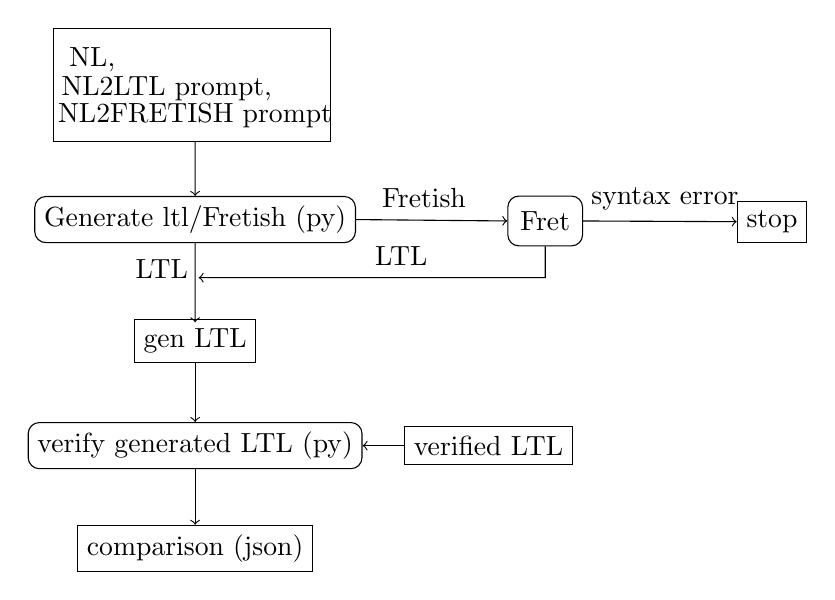
\begin{tikzpicture}[scale=0.9]
  \node[draw, rounded corners] (node1) at (1.8,2.9) {Generate ltl/Fretish (py)};
  \node at (0.35,5.15) {NL,};
  \node at (1.33,2.2) {LTL};
  \node at (1.4,4.74) {NL2LTL prompt,};
  \node at (1.8,4.36) {NL2FRETISH prompt};
  \draw (-0.2,5.6) rectangle (3.71,4);
  \draw[->] (1.8,4) -- (node1.north);
  \draw[->] (node1.south) -- (1.8,1.45);
  \node[draw, shape=rectangle, rounded corners, minimum width=27pt, minimum height=18pt] (node2) at (6.74,2.88) {Fret};
  \draw[->] (node1.east) -- (node2.west);
  \node at (5.03,3.21) {Fretish};
  \node at (4.71,2.38) {LTL};
  \node at (8.43,3.19) {syntax error};
  \draw[->] (node2.south) -- (6.74,2.08) .. controls (5.04,2.08) and (3.71,2.08) .. (1.85,2.08);
  \node[draw] (node5) at (5.94,-0.29) {verified  LTL};
  \node[draw] (node3) at (1.8,1.19) {gen LTL};
  \node[draw, rounded corners] (node4) at (1.8,-0.29) {verify generated LTL (py)};
  \draw[->] (node3.south) -- (node4.north);
  \draw[->] (node5.west) -- (node4.east);
  \node[draw] (node6) at (1.8,-1.74) {comparison (json)};
  \draw[->] (node4.south) -- (node6.north);
  \node[draw] (node7) at (9.94,2.87) {stop};
  \draw[->] (node2.east) -- (node7.west);
\end{tikzpicture}
\end{center}
\end{frame}

\begin{frame}{Verifying LTL}
    \begin{center}
        
\includegraphics[width=0.55\textwidth]{images/verifing.png}
    \end{center}
%     \begin{center}
%         \begin{tikzpicture}[scale=1]
%   \node[draw] at (0.89,2.71) {Gen LTL};
%   \node[draw] at (3.4,2.71) {Verified LTL};
%   \node[draw] at (4.59,-4.47) {Verified LTL};
%   \node[draw, rounded corners] (node1) at (2.09,1.31) {var  extract()};
%   \draw (0.89,2.47) -- (0.89,2) -- (2.09,2) -- (node1.north);
%   \draw[arrows=-Stealth] (3.4,2.47) -- (3.4,2) -- (2.09,2) -- (node1.north);
%   \node[draw, rounded corners] (node2) at (2.09,-0.04) {compare vars()};
%   \node[draw, rounded corners] (node3) at (6,-0.04) {all-MiniLM-L6-v2};
%   \draw[arrows=-Stealth] (node1.south) -- (node2.north);
%   \draw[arrows=-Stealth] (node3.west) -- (node2.east);
%   \node[draw, rounded corners] (node4) at (0.16,-1.5) {replace with verified};
%   \node[draw, rounded corners] at (4.49,-1.5) {replace with !verified-var};
%   \node[draw, minimum width=29pt, minimum height=14pt] at (7.71,-1.47) {error};
%   \draw[arrows=-Stealth] (2.09,-0.33) .. controls (2.09,-1.22) and (0,-0.59) .. (0,-1.22);
%   \draw[arrows=-Stealth] (2.09,-0.33) .. controls (2.09,-1.22) and (4.49,-0.62) .. (4.49,-1.22);
%   \draw[arrows=-Stealth] (2.09,-0.33) .. controls (2,-0.88) and (7.71,-0.5) .. (7.71,-1.22);
%   \node[draw, rounded corners, minimum width=60pt, minimum height=19pt] (node5) at (2.38,-3.5) {substitute};
%   \draw (node4.south) -- (0.16,-2.5) -- (2.38,-2.5) -- (2.38,-2.76);
%   \draw[arrows=-Stealth] (4.49,-1.78) -- (4.49,-2.5) -- (2.38,-2.5) -- (node5.north);
%   \node[draw] (node6) at (1.35,-4.5) {new  gen LTL};
%   \draw[arrows=-Stealth] (node5.south) -- (node6.north);
%   \node[draw, rounded corners] (node8) at (2.59,-5.77) {Compare LTLs};
%   \draw (node6.south) -- (1.35,-5.16) -- (2.59,-5.18) -- (2.59,-5.5);
%   \draw[arrows=-Stealth] (4.59,-4.71) -- (4.59,-5.16) -- (2.59,-5.18) -- (2.59,-5.5);
%   \node[draw, rounded corners] (node7) at (6.29,-5.77) {Spot};
%   \draw[arrows=-Stealth] (node7.west) -- (node8.east);
%   \node[draw] at (0.48,-7.24) {Valid};
%   \node[draw, rounded corners] (node9) at (3.84,-7.21) {get counter example};
%   \draw[arrows=-Stealth] (node8.south) -- (2.59,-6.5) -- (0.48,-6.5) -- (0.48,-7);
%   \draw[arrows=-Stealth] (node8.south) -- (2.59,-6.5) -- (3.84,-6.5) -- (3.84,-6.94);
%   \node at (1.42,-6.35) {true};
%   \node at (3.19,-6.35) {false};
%   \draw[arrows=-Stealth] (node7.south) -- (6.29,-7.21) -- (5.5,-7.21);
%   \node[draw] (node10) at (3.84,-8.27) {counter example};
%   \draw[arrows=-Stealth] (node9.south) -- (node10);
% \end{tikzpicture}
%     \end{center}
\end{frame}

\begin{frame}{Results}
    \begin{itemize}
        \item Total: 920
        \item True: 675
        \item False: 228
        \item errors: 7 (response contained other data)
        \item More results \href{https://melchizedektp.github.io/nl2ltl/}{Here}.
    \end{itemize}
\end{frame}

\begin{frame}{Traces}
    
\end{frame}
